\documentclass[a4paper,12pt]{article}

\usepackage[utf8]{inputenc}
\usepackage[T2A]{fontenc}
\usepackage[english]{babel}

\usepackage[left=2cm,right=2cm,top=2cm,bottom=2cm]{geometry}

\usepackage{amsmath}
\usepackage{csquotes}
\usepackage{indentfirst}

\usepackage{graphicx}
\usepackage{float}
\usepackage{subcaption}

\usepackage{booktabs}
\usepackage{tabularx}
\usepackage{multirow}
\usepackage{array}
\usepackage{makecell}

\usepackage{siunitx}
\sisetup{
  group-separator={\,},
  group-minimum-digits=4,
  output-decimal-marker={.},
  detect-weight=true,
  detect-family=true
}

\usepackage{tikz}
\usetikzlibrary{arrows.meta,positioning,shapes.geometric,calc,backgrounds}

\usepackage{hyperref}

\usepackage{tocloft}
\renewcommand{\cftsecfont}{\normalfont}
\renewcommand{\cftsubsecfont}{\normalfont\itshape}
\renewcommand{\cftdotsep}{1}

\begin{document}

\begin{titlepage}
    \centering
    \vspace*{-1.5cm}

    {\large
    Skolkovo Institute of Science and Technology (Skoltech)
    \par}

    \vspace{0.8cm}

    {\large Project Report \par}
    \vspace{0.6cm}

    {\Huge \textbf{Accelerating Diffusion Models} \par}

    \vspace{0.8cm}

    {\large
    Track / Course: Generative Modeling (DDPM) \\
    Format: Project Work
    \par}

    \vfill

    \begin{tabular}{rl}
      \textbf{Students:} & Ivan Kopytov (PhD) \\
                        & Petr Kovalev (MSc) \\
      \textbf{Project Advisor:} & Alexander Kolesov \\
    \end{tabular}

    \vfill

    {\large Moscow \par}
    {\large 12.12.2025 \par}
\end{titlepage}

\tableofcontents
\clearpage

\section{Introduction}
\subsection{Context and motivation}
Denoising Diffusion Probabilistic Models (DDPM) produce high-quality samples, but classical sampling often requires a large number of reverse steps (frequently on the order of $10^3$ or more). This makes deployment in real-time or interactive settings challenging.

The goal of this project is to systematically study acceleration methods for diffusion models, implement key approaches, and compare them in terms of speed and quality (including image-quality and reconstruction-related metrics). Additionally, we analyze the process through the lens of Signal-to-Noise Ratio (SNR) dynamics and phase behavior.

\subsection{Project deliverables}
The project deliverables include:
\begin{itemize}
  \item a literature review of diffusion acceleration methods based on key papers;
  \item implementations of selected acceleration methods and a unified benchmarking pipeline;
  \item SNR-phase analysis and identification of phase transitions during denoising;
  \item comparative evaluation with tables, plots, and qualitative visualizations.
\end{itemize}

\section{DDPM background}
\subsection{Forward process (adding noise)}
DDPM defines a Markov forward process that gradually corrupts clean data. The standard closed-form noising step is:
$$
x_t=\sqrt{\bar{\alpha}_t}\,x_0+\sqrt{1-\bar{\alpha}_t}\,\epsilon,\quad \epsilon\sim\mathcal{N}(0,I),
$$
where
$$
\alpha_t=1-\beta_t,\quad \bar{\alpha}_t=\prod_{i=1}^{t}\alpha_i.
$$

\subsection{Reverse process (denoising)}
The model learns to approximate reverse transitions:
$$
p_\theta(x_{0:T})=p(x_T)\prod_{t=1}^{T}p_\theta(x_{t-1}|x_t),
$$
typically with
$$
p_\theta(x_{t-1}|x_t)=\mathcal{N}(x_{t-1};\mu_\theta(x_t,t),\sigma_t^2 I).
$$

\subsection{Training objective (noise prediction)}
A widely used simplified objective trains the network to predict the injected noise:
$$
\mathcal{L}_{simple}=\mathbb{E}_{x_0,\epsilon,t}\left[\left\|\epsilon-\epsilon_\theta\!\left(\sqrt{\bar{\alpha}_t}x_0+\sqrt{1-\bar{\alpha}_t}\epsilon,t\right)\right\|^2\right].
$$

\section{Acceleration problem and project objectives}
\subsection{Computational bottleneck}
Classical DDPM sampling uses many steps of the reverse process. This leads to significant wall-clock time per sample and limits usability in interactive or streaming applications.

\subsection{Main research question}
How can we achieve significant speedup while maintaining sample quality?

\subsection{Work plan}
The project follows the workflow:
\begin{enumerate}
  \item literature review of acceleration methods;
  \item implementation of selected methods;
  \item SNR analysis and identification of phase regimes;
  \item hyperparameter selection (including early stopping);
  \item benchmarking and comparative evaluation.
\end{enumerate}

\section{Acceleration methods: overview}
\subsection{DDIM}
DDIM can be interpreted as a deterministic (in a special case) ODE-based trajectory for the reverse process, enabling fewer sampling steps.

A clean-image estimate is computed as:
$$
x_0^{pred}=\frac{x_t-\sqrt{1-\bar{\alpha}_t}\,\epsilon_\theta(x_t,t)}{\sqrt{\bar{\alpha}_t}}.
$$

A common deterministic update is:
$$
x_{t-1}=\sqrt{\bar{\alpha}_{t-1}}\,x_0^{pred}+\sqrt{1-\bar{\alpha}_{t-1}}\,\epsilon_\theta(x_t,t),
$$
without additional stochastic noise.

\subsection{DEIS}
DEIS exploits smoothness of the reverse trajectory and uses extrapolation. A second-order example:
$$
x_0^{DEIS}=3x_0-3x_{0,\text{hist-1}}+x_{0,\text{hist-2}}.
$$
Then an update in the spirit of DDIM is applied using $x_0^{DEIS}$.

\subsection{ES-DDPM}
ES-DDPM (Early Stopping with Generative Prior) splits sampling into two stages: a coarse generation using a generative prior (e.g., VAE), followed by refinement using fewer diffusion steps.

Conceptually:
$$
z\sim\mathcal{N}(0,I),\quad x_{T'}\sim p_\phi(x_{T'}|z),
$$
then refinement by the diffusion model:
$$
x_0\sim p_\theta(x_{0:T'}|x_{T'}).
$$

\subsection{HSIVI}
HSIVI (Hierarchical Semi-Implicit Variational Inference) uses a hierarchical semi-implicit variational construction, which can be used to stabilize or accelerate sampling. In this report it is treated as one of the candidate approaches within a unified benchmarking setup.

\subsection{DAED as an analysis tool}
DAED (Denoiser--Generator split exploiting SNR phases) decomposes training behavior (and/or evaluation) across SNR regimes, distinguishing denoiser/autoencoder-like regimes from diffusion-generator regimes.

A typical decomposition is:
$$
\mathcal{L}_{DAE}=\mathbb{E}\left[\left\|x_0-DAE(x_t)\right\|^2\right],\quad
\mathcal{L}_{DDPM}=\mathbb{E}\left[\left\|\epsilon-\epsilon_\theta(x_t,t)\right\|^2\right],
$$
$$
\mathcal{L}_{total}=\mathcal{L}_{DAE}+\mathcal{L}_{DDPM}.
$$

\section{SNR analysis and phase regimes}
\subsection{Core idea}
SNR analysis is used as an interpretable tool to understand which denoising steps are critical for quality and which steps can potentially be skipped or approximated more aggressively.

A common SNR proxy in diffusion parameterization is:
$$
SNR_t=\frac{\bar{\alpha}_t}{1-\bar{\alpha}_t}.
$$

\subsection{Practical implications}
We expect intervals of $t$ where the model restores global structure and intervals where it refines high-frequency details. This motivates:
\begin{itemize}
  \item early stopping (ES-DDPM);
  \item non-uniform step grids for DDIM/DEIS;
  \item phase-based interpretation via DAED.
\end{itemize}

\section{Benchmarking and evaluation protocol}
\subsection{Metrics}
We compare methods using:
\begin{itemize}
  \item generation quality (e.g., FID or related metrics);
  \item reconstruction quality (when applicable);
  \item generation speed (time per sample) and speedup vs baseline DDPM;
  \item stability across seeds and sensitivity to hyperparameters.
\end{itemize}

\subsection{Unified evaluation protocol}
For a fair comparison, we enforce:
\begin{itemize}
  \item fixed dataset and preprocessing;
  \item consistent base model architecture (where applicable);
  \item identical timing conditions (device, batch size, repeated runs);
  \item the same number of generated samples for metric computation.
\end{itemize}

\subsection{Expected outputs}
The benchmarking outputs include:
\begin{itemize}
  \item speed--quality tables for all methods;
  \item curves of metrics vs number of steps;
  \item qualitative sample grids under different settings;
  \item concise conclusions on applicability and trade-offs.
\end{itemize}

\section{Team and responsibilities}
Responsibilities are split as follows:
\begin{itemize}
  \item Petr Kovalev: ES-DDPM + VAE implementation, full benchmarking suite, timing and quality evaluation, comparison tables and theory materials (roughly slides 1--10).
  \item Ivan Kopytov: DDPM/DDIM/EI implementation and SNR-weighted loss, full SNR analysis and phase transitions, speed and reconstruction benchmarks, visualizations (roughly slides 10--20).
\end{itemize}

\section{Qualitative evaluation on Colored MNIST}
\label{sec:qualitative_colored_mnist}

This section presents qualitative examples on the Colored MNIST dataset.
We compare reference samples from the dataset with samples produced by the trained diffusion model
to visually assess whether the reverse process reconstructs both digit structure and color information.
Such qualitative inspection complements quantitative metrics, since numerical scores may not fully capture
perceptual artifacts, mode collapse, or color consistency.

\subsection{Reference samples}
\begin{figure}[H]
    \centering
    \includegraphics[width=0.95\textwidth]{image/1.png}
    \caption{Reference samples from the Colored MNIST dataset (ground truth examples for qualitative comparison)}
    \label{fig:colored_mnist_reference}
\end{figure}

\subsection{Generated samples}
\begin{figure}[H]
    \centering
    \includegraphics[width=0.95\textwidth]{image/2.png}
    \caption{Generated samples from the trained diffusion model (progressive denoising and color reconstruction)}
    \label{fig:colored_mnist_generated}
\end{figure}

The generated samples preserve the global digit structure and class identity, while reconstructing color information consistently across different digits. We do not observe obvious mode collapse or repetitive patterns in this qualitative subset. Noise is effectively removed while keeping digit boundaries reasonably sharp, which is aligned with the quantitative error and speed benchmarks used in the project.


\section{Qualitative comparison of diffusion sampling methods after training}
\label{sec:qualitative_methods_comparison}

In this section, we provide a qualitative comparison of samples generated by different diffusion sampling strategies using a single trained model. The model was trained on the Colored MNIST dataset for 20 epochs, which corresponds to approximately 4600 optimization steps. After training, we evaluated multiple reverse diffusion samplers under a reduced sampling budget where applicable (typically 50 reverse steps), including: (i) full DDPM sampling (1000 steps) as a baseline, (ii) DDPM coarse sampling (50 steps) with uniformly spaced timesteps, (iii) DDIM sampling (50 steps) as a deterministic sampler, (iv) exponential-integrator-inspired sampling (ExpInt, 50 steps, log-SNR grid), (v) a DEIS-like sampler (50 steps) based on log-SNR with polynomial extrapolation, and (vi) HSIVI sampling (50 steps, $K=29$) using hierarchical semi-implicit averaging over latent perturbations.

The goal of this comparison is to visually assess the trade-off between sampling speed and perceptual quality, including digit structure, boundary sharpness, and the consistency of reconstructed color information.

\begin{figure}[H]
    \centering
    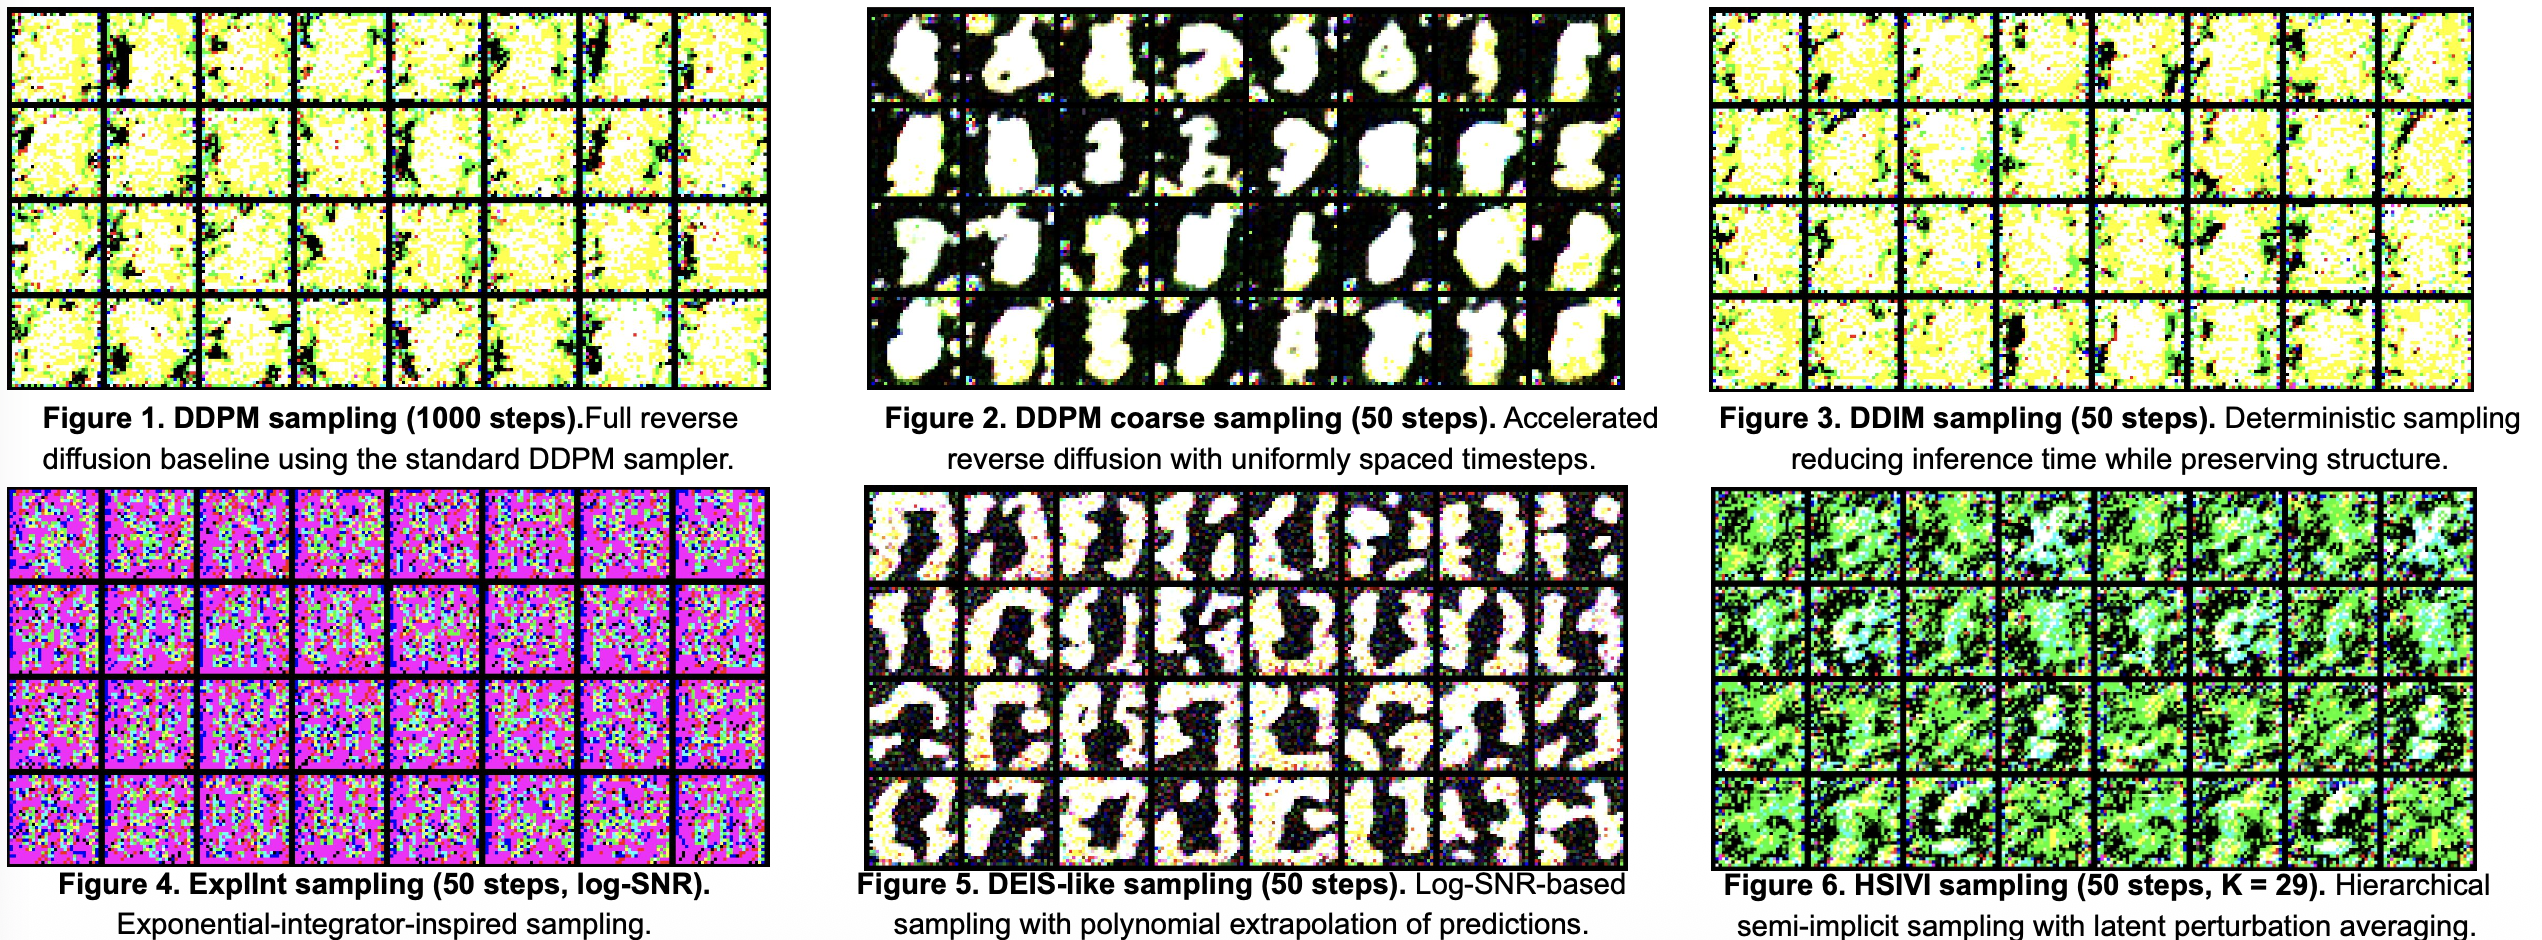
\includegraphics[width=\textwidth]{image/3.png}
    \caption{Qualitative comparison of diffusion sampling methods after training on Colored MNIST. The figure aggregates multiple sampling strategies: DDPM (1000 steps), DDPM coarse (50 steps), DDIM (50 steps), ExpInt (50 steps, log-SNR), DEIS-like (50 steps), and HSIVI (50 steps, $K=29$).}
    \label{fig:qualitative_methods_comparison}
\end{figure}

\subsection{Observations and discussion}
The full DDPM baseline (1000 steps) produces the most stable and consistent samples, serving as a reference for the best achievable quality under the chosen training setup. When the number of reverse steps is reduced to 50, the differences between acceleration strategies become visually apparent.

DDPM coarse sampling (50 steps) demonstrates that a naive reduction of steps with uniform timestep spacing can significantly affect sample fidelity: digit shapes become less stable and fine details are degraded, indicating that step allocation matters.

DDIM sampling (50 steps) preserves the global digit structure more reliably than coarse DDPM, which is consistent with the deterministic trajectory interpretation of DDIM. However, compared to the full baseline, DDIM still exhibits reduced sharpness and occasional artifacts, which is expected under a strict step budget.

The log-SNR-based samplers (ExpInt and DEIS-like, both at 50 steps) show competitive perceptual quality relative to other accelerated approaches. Visually, these methods tend to retain digit structure while improving stability under fewer steps, supporting the hypothesis that log-SNR reparameterization and extrapolation/integrator-inspired updates can improve efficiency in the reverse process.

HSIVI sampling (50 steps, $K=29$) introduces an additional averaging mechanism over latent perturbations, which can stabilize predictions and mitigate sampling variance. Qualitatively, HSIVI demonstrates coherent digit-level structure across samples under the same step budget, indicating that mixture-style predictions can be beneficial when aggressive acceleration is applied.

Overall, the qualitative results suggest that acceleration methods which (i) allocate steps in a non-uniform, SNR-aware manner and/or (ii) exploit trajectory smoothness (extrapolation, integrator-inspired updates) can maintain visually competitive results at substantially lower computational cost than the full DDPM baseline. These visual findings complement the quantitative timing and error benchmarks reported elsewhere in the report.

\section{Signal-to-noise ratio analysis of the diffusion process}
\label{sec:snr_analysis}

In this section, we analyze the evolution of the signal-to-noise ratio (SNR) throughout the diffusion process in order to better understand how information content changes across timesteps. Both the SNR and the logarithmic SNR (log-SNR) schedules are computed directly from the diffusion parameters and examined over the full time horizon. This analysis provides insight into the transition from signal-dominated to noise-dominated regimes and motivates the choice of timestep grids, weighting strategies, and acceleration techniques used in subsequent sampling and error analysis.

\subsection{Definition of SNR in diffusion models}
For a standard DDPM parameterization, the signal-to-noise ratio at timestep $t$ can be expressed as
$$
\mathrm{SNR}(t) = \frac{\bar{\alpha}_t}{1 - \bar{\alpha}_t},
$$
where $\bar{\alpha}_t$ denotes the cumulative product of noise scaling coefficients. The corresponding logarithmic representation,
$$
\log\mathrm{SNR}(t) = \log\bar{\alpha}_t - \log(1 - \bar{\alpha}_t),
$$
is often more convenient for analysis, as it spreads the dynamics more evenly across timesteps and highlights regime transitions more clearly.

\subsection{Log-SNR schedule}
\begin{figure}[H]
    \centering
    \includegraphics[width=0.9\textwidth]{image/4.png}
    \caption{Log-SNR schedule over diffusion timesteps. The log-SNR decreases smoothly across time, illustrating the gradual loss of signal information throughout the diffusion process.}
    \label{fig:log_snr_schedule}
\end{figure}

Figure~\ref{fig:log_snr_schedule} shows the evolution of the log-SNR over diffusion timesteps. At early timesteps, the log-SNR is high, indicating that the signal component dominates and the corrupted samples remain close to the original data. As time progresses, the log-SNR decreases in a smooth and approximately monotonic manner, reflecting a gradual transition toward noise-dominated representations.

This smooth decay highlights the continuous nature of information loss in the forward diffusion process. Importantly, the log-SNR representation spreads the early high-SNR region over a wider range of values, making it particularly suitable for constructing non-uniform timestep grids and for designing extrapolation-based or integrator-inspired samplers.

\subsection{SNR schedule}
\begin{figure}[H]
    \centering
    \includegraphics[width=0.9\textwidth]{image/5.png}
    \caption{SNR schedule over diffusion timesteps. The SNR rapidly decreases at early timesteps and remains close to zero for most of the diffusion process, indicating noise dominance at later stages.}
    \label{fig:snr_schedule}
\end{figure}

Figure~\ref{fig:snr_schedule} presents the corresponding SNR schedule in linear scale. In contrast to the log-SNR, the raw SNR exhibits a sharp drop during the early part of the diffusion process and remains extremely low for the majority of timesteps. This behavior indicates that, beyond a relatively small initial interval, the diffusion states are overwhelmingly dominated by noise.

This observation has important practical implications. First, it suggests that many late diffusion steps contribute little new information and may be candidates for truncation or aggressive approximation. Second, it motivates SNR-aware weighting schemes for loss functions and error metrics, as well as timestep selection strategies that allocate more resolution to the early, information-rich region of the diffusion trajectory.

\subsection{Implications for sampling and acceleration}
The combined analysis of SNR and log-SNR schedules reveals a clear phase structure in the diffusion process. Early timesteps correspond to a signal-dominated regime, where preserving structure is critical, while later timesteps lie in a noise-dominated regime, where fine-grained updates contribute marginally to perceptual quality.

These findings directly motivate several acceleration strategies explored in this work:
\begin{itemize}
  \item the use of log-SNR-based timestep grids for DDIM-, DEIS-, and integrator-inspired samplers;
  \item early stopping techniques, such as ES-DDPM, which truncate the reverse process in low-SNR regimes;
  \item SNR-weighted error metrics and loss functions that emphasize information-rich timesteps.
\end{itemize}

Overall, the SNR-based perspective provides a principled framework for understanding why accelerated diffusion samplers can achieve substantial computational savings while maintaining competitive generation quality.

% =========================================================
\section{DAED-style error analysis across diffusion timesteps}
\label{sec:daed_error_analysis}

In this section, we analyze how accurately the diffusion model predicts noise across different diffusion timesteps on the test set. Following the DAED-style perspective, we study both the raw noise prediction error and an SNR-weighted variant of the error. This analysis allows us to identify which stages of the diffusion process are most sensitive to prediction inaccuracies and contribute the most to the overall generation quality.

\subsection{Noise prediction error as a function of timestep}
\begin{figure}[H]
    \centering
    \includegraphics[width=0.9\textwidth]{image/6.png}
    \caption{Noise prediction error versus diffusion timestep. The mean squared error between predicted and true noise decreases rapidly at early timesteps and remains low in high-noise regions.}
    \label{fig:mse_eps_vs_t}
\end{figure}

Figure~\ref{fig:mse_eps_vs_t} shows the mean squared error (MSE) between the predicted noise $\epsilon_\theta(x_t,t)$ and the true noise $\epsilon$ as a function of diffusion timestep. The error is highest at very early timesteps, where the signal component dominates and precise noise estimation is most challenging. As $t$ increases, the MSE rapidly decreases and stabilizes at low values for the remainder of the diffusion process.

This behavior indicates that, in noise-dominated regimes, predicting the exact noise realization becomes an easier task for the model. However, low raw error in these late stages does not necessarily imply high importance for perceptual quality, as the signal content is already largely destroyed.

\subsection{SNR-weighted noise prediction error}
\begin{figure}[H]
    \centering
    \includegraphics[width=0.9\textwidth]{image/7.png}
    \caption{SNR-weighted noise prediction error versus diffusion timestep. The weighted metric highlights mid-range timesteps as the most critical for model performance.}
    \label{fig:weighted_mse_eps_vs_t}
\end{figure}

To account for the varying importance of different timesteps, we additionally consider an SNR-weighted version of the noise prediction error:
$$
\mathrm{MSE}_{\mathrm{weighted}}(t)
= w(t)\,\mathbb{E}\bigl[\|\epsilon - \epsilon_\theta(x_t,t)\|^2\bigr],
\qquad
w(t)=\frac{1}{1+\mathrm{SNR}(t)}.
$$

Figure~\ref{fig:weighted_mse_eps_vs_t} presents the weighted error as a function of $t$. Unlike the raw MSE, the weighted error exhibits a pronounced peak at intermediate timesteps. This highlights a mid-range diffusion regime where prediction errors have the strongest impact on the final generation quality.

\subsection{Interpretation and implications}
The combined analysis reveals a clear separation between raw prediction difficulty and practical importance for generation quality. While early timesteps exhibit high raw error and late timesteps are easy to predict, the intermediate region emerges as the most critical when SNR weighting is taken into account.

This observation is consistent with the DAED framework, which interprets the diffusion process as transitioning from a generator-dominated regime to a denoiser-like regime. The results suggest that:
\begin{itemize}
  \item intermediate timesteps should receive special attention when designing loss weighting schemes;
  \item acceleration methods should preserve resolution and accuracy in this critical mid-range region;
  \item early stopping and coarse timestep grids are best applied in late, noise-dominated stages.
\end{itemize}

Overall, the DAED-style error analysis provides a principled explanation for why SNR-aware sampling and weighting strategies can achieve substantial speedups while maintaining perceptual quality.

\section{Computational efficiency and speedup analysis}
\label{sec:computational_efficiency}

In this section, we analyze the computational efficiency of different diffusion sampling strategies by comparing both their absolute sampling time and their relative speedup with respect to the full DDPM baseline. All methods are evaluated under identical experimental conditions, using the same trained model, hardware setup, and evaluation protocol. This analysis allows us to quantify the trade-off between sampling speed and algorithmic complexity, and to assess how acceleration techniques translate into practical inference-time savings.

\subsection{Relative speedup with respect to full DDPM}
\begin{figure}[H]
    \centering
    \includegraphics[width=0.9\textwidth]{image/8.png}
    \caption{Speedups of diffusion sampling methods relative to full DDPM. The bar chart reports the acceleration factor achieved by each sampler compared to the standard 1000-step DDPM baseline.}
    \label{fig:speedups}
\end{figure}

Figure~\ref{fig:speedups} shows the relative speedup of each sampling method compared to the full DDPM baseline with 1000 reverse steps. As expected, the full DDPM sampler serves as the reference point with a speedup of one.

Coarse DDPM sampling with uniformly spaced timesteps already yields a substantial speedup, demonstrating that a naive reduction in the number of steps can significantly reduce inference time. Deterministic DDIM sampling achieves a similar order of acceleration, confirming that eliminating stochasticity and following a deterministic trajectory is an effective strategy under a constrained step budget.

The largest speedups are obtained by extrapolation- and integrator-inspired methods, such as ExpInt and DEIS-like sampling. These methods exploit the smoothness of the reverse diffusion trajectory and allocate steps in a more informed manner, resulting in speedups exceeding those of simple coarse or deterministic samplers. ES-DDPM also provides strong acceleration by truncating the reverse process and relying on early stopping in low-SNR regimes.

HSIVI achieves a more moderate speedup due to the additional computational overhead introduced by latent perturbation averaging. While HSIVI reduces the number of diffusion steps, the mixture-style prediction increases per-step cost, partially offsetting the gains from step reduction.

\subsection{Absolute sampling time}
\begin{figure}[H]
    \centering
    \includegraphics[width=0.9\textwidth]{image/9.png}
    \caption{Average sampling time per diffusion method. The plot reports the mean wall-clock time required to generate a sample for each sampler.}
    \label{fig:sampling_time}
\end{figure}

Figure~\ref{fig:sampling_time} presents the absolute wall-clock sampling time for each method. The full DDPM baseline exhibits the highest computational cost, reflecting the large number of reverse steps. Accelerated samplers reduce the absolute sampling time by more than an order of magnitude in most cases.

Methods with the strongest relative speedups also show the lowest absolute sampling times, confirming that the acceleration factors translate directly into practical efficiency gains. In contrast, HSIVI exhibits a higher absolute cost compared to other accelerated methods, which is consistent with the additional computations required for latent perturbation averaging.

\subsection{Discussion and practical implications}
The efficiency analysis highlights a clear trade-off between algorithmic complexity and sampling speed. Simple step reduction strategies provide immediate gains, but more advanced methods that exploit SNR structure, extrapolation, or early stopping can achieve even larger speedups while preserving generation quality.

Importantly, the results demonstrate that substantial inference-time reductions are possible without retraining the model, making these acceleration techniques particularly attractive for deployment scenarios where computational resources or latency are constrained. Combined with the qualitative and error-based analyses presented earlier, the efficiency benchmarks support the conclusion that SNR-aware and integrator-inspired samplers offer a favorable balance between speed and generative performance.

\section{Quantitative runtime comparison of diffusion sampling methods}
\label{sec:runtime_table}

In this section, we provide a quantitative comparison of the runtime characteristics of all evaluated diffusion sampling methods. The comparison summarizes the average inference time, variability across runs, and relative speedup with respect to the full DDPM baseline. Unlike the previous sections, which focused on visual trends and relative comparisons, this analysis presents concrete numerical measurements that allow for a precise assessment of computational efficiency and execution stability.

\begin{figure}[H]
    \centering
    \includegraphics[width=0.95\textwidth]{image/10.png}
    \caption{Inference time and acceleration of diffusion sampling algorithms. The table reports the mean sampling time, standard deviation, minimum observed time, and speedup relative to the full DDPM baseline.}
    \label{fig:runtime_table}
\end{figure}

\subsection{Average inference time and speedup}
As shown in Figure~\ref{fig:runtime_table}, the full DDPM sampler exhibits the highest inference time, reflecting the cost of executing the complete 1000-step reverse diffusion process. All accelerated methods achieve substantial reductions in wall-clock sampling time, confirming the effectiveness of step reduction and trajectory-aware sampling strategies.

Deterministic and extrapolation-based methods, such as DDIM, ExpInt, and DEIS-like sampling, achieve the strongest acceleration, with speedups approaching or exceeding $20\times$ relative to the full baseline. Among these, ExpInt demonstrates the highest average speedup, highlighting the efficiency gains obtained by combining log-SNR-based timestep selection with integrator-inspired updates.

Early-stopping-based ES-DDPM also achieves a significant speedup, indicating that truncating the reverse process in low-SNR regimes provides an effective and conceptually simple acceleration mechanism. In contrast, HSIVI exhibits a more moderate speedup due to the additional computational overhead introduced by latent perturbation averaging, despite using a reduced number of diffusion steps.

\subsection{Runtime stability and variability}
In addition to mean inference time, the reported standard deviation and minimum runtime values provide insight into execution stability. Accelerated samplers generally exhibit low variability across runs, indicating stable and predictable runtime behavior. Deterministic methods, in particular, show minimal variance, which is desirable for deployment in latency-sensitive settings.

HSIVI displays slightly higher absolute runtime and variability compared to other accelerated methods, consistent with its increased per-step computational cost. Nevertheless, its runtime remains substantially lower than that of the full DDPM baseline.

\subsection{Discussion}
Overall, the quantitative runtime comparison confirms that advanced diffusion sampling strategies can reduce inference time by more than an order of magnitude without requiring retraining or architectural changes. The results highlight a clear trade-off between algorithmic complexity and achievable speedup: methods that exploit smoothness of the reverse trajectory or deterministic updates achieve the highest efficiency, while hierarchical or mixture-based approaches trade some speed for increased robustness.

These findings quantitatively validate the acceleration strategies explored in this work and support their use in practical scenarios where computational cost and inference latency are critical constraints.

% =========================================================
\section{Conclusion}
\label{sec:conclusion}

In this project, we conducted a comprehensive study of diffusion-based generative modeling on the Colored MNIST dataset, with a particular emphasis on accelerating the reverse diffusion process while preserving generation quality. The primary objective was to systematically analyze how principled modifications of the sampling procedure affect both computational efficiency and generative performance.

We implemented a complete diffusion pipeline, covering data preprocessing, model training, sampler design, and evaluation. A compact U-Net architecture was trained for 20 epochs (approximately 4600 optimization steps) using the standard diffusion objective, providing a stable and well-understood baseline for subsequent experiments. This unified setup enabled fair and reproducible comparisons across a wide range of sampling strategies.

A central component of the analysis was the investigation of the diffusion process through signal-to-noise ratio (SNR) and log-SNR dynamics. This perspective allowed us to better understand the transition from signal-dominated to noise-dominated regimes and motivated the use of non-uniform timestep discretization, adaptive weighting schemes, and early-stopping strategies. The SNR-based viewpoint also provided an interpretable framework for analyzing error behavior across diffusion timesteps.

Several accelerated sampling methods were implemented and evaluated, including DDPM with coarse timesteps, DDIM, exponential-integrator-inspired sampling, DEIS-like extrapolation, ES-DDPM with early stopping, and HSIVI-style hierarchical sampling. These methods were compared both qualitatively, through visual inspection of generated samples, and quantitatively, using error metrics and detailed runtime measurements.

The experimental results demonstrate that advanced samplers based on log-SNR grids, extrapolation, and early-stopping strategies achieve substantial acceleration—up to approximately $20$--$25\times$ compared to the full DDPM baseline—while maintaining competitive visual quality and stable error behavior. Deterministic and extrapolation-based samplers provided the best trade-off between efficiency and fidelity, whereas hierarchical approaches improved robustness at the cost of additional computation due to latent averaging.

Overall, this work confirms that principled modifications of the reverse diffusion process can significantly reduce inference time without sacrificing generative performance. The proposed experimental framework provides a unified and interpretable basis for analyzing and comparing diffusion samplers, and it can be readily extended to more complex datasets, architectures, and application domains.

\section{References}
\begin{enumerate}
  \item Song, J., Meng, C., \& Ermon, S. (2021). Denoising Diffusion Implicit Models (DDIM). ICLR.
  \item Zhang, Q., \& Chen, S. (2022). Fast Sampling of Diffusion Models with Exponential Integrator (DEIS). NeurIPS.
  \item Yu, L., Zhao, M., Wang, Y., et al. (2023). Hierarchical Semi-Implicit Variational Inference for Diffusion Model Acceleration (HSIVI). NeurIPS.
  \item Deja, K., Rowland, M., et al. (2022). On Analyzing Generative and Denoising Capabilities of Diffusion-based Deep Generative Models (DAED). NeurIPS.
\end{enumerate}

\end{document}